% Consider laminar flow between two parallel plates (Fig. 1). Plates extend infinitely in x and
% z directions. The following assumptions are made:
% • the flow is at steady state (no time dependency)
% • the fluid is incompressible, ideal and Newtonian
% • the temperature of the bottom plate is Tb and the upper plate is at temperature Tu
% • vy = vz = 0
% • vx = vx(y), T = T(y)
% Figure 1: Problem statement: fluid flow between two parallel plates. The bottom plate is
% fixed, the upper plate is moving horizontally with velocity uw. The fluid is incompressible
% and Newtonian.


\section{}
\textit{Write down the full set of governing equations (continuity, momentum and energy).}

\begin{figure}[h]
    \centering
    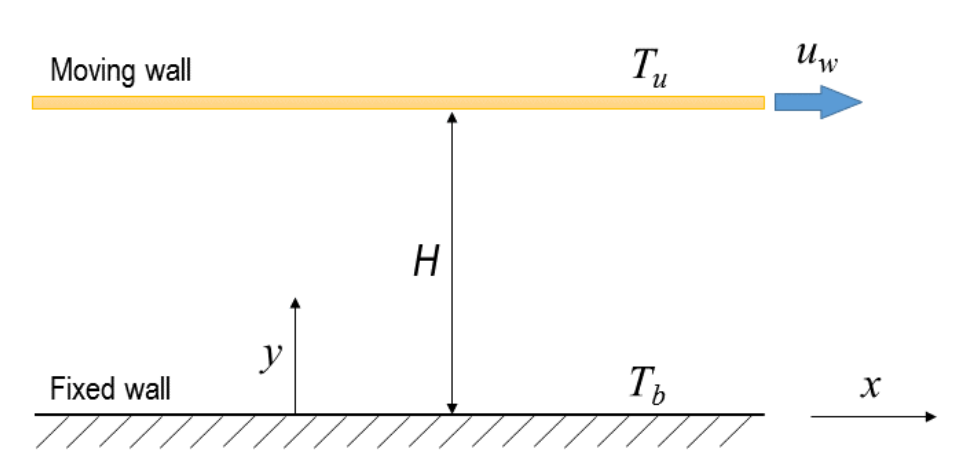
\includegraphics[width=0.5\textwidth]{Questions/Figures/Q1 diagram.png}
    \caption{Fluid flow betweeen parallel plates. The bottom plate is fixed, the upper plate is moving horizontally with velocity $u_w$. THe fluid is incompressible and Newtonian.}
    \label{fig:Q1 diagram}
\end{figure}

\subsection*{Solution}
We first begin with continuity, 
\begin{align*}
    \Aboxed{\frac{\partial \rho}{\partial t} + \vec{u} \cdot \nabla \rho + \rho (\nabla \cdot \vec{u}) &= 0}
\end{align*}
then, the momentum equation,
\begin{align*}
    \Aboxed{\frac{\partial}{\partial t} (\rho u_i) + \frac{\partial}{\partial x_j} (\rho u_i u_j) &= -\frac{\partial P}{\partial x_i} + \frac{\partial}{\partial x_j} \left[ \mu \left( \frac{\partial u_i}{\partial x_j} + \frac{\partial u_j}{\partial x_i} \right) \right] - \frac{\partial}{\partial x_i} \left(\frac{2}{3} \mu \frac{\partial u_k}{\partial x_k} \right) + \rho b_i}
\end{align*}
lastly, the energy equation,
\begin{align*}
    \Aboxed{\rho C_p \left(\frac{\partial T}{\partial t} + \vec{v} \cdot \nabla T \right) &= k \nabla^2 T + \frac{\mu}{2} \Phi^2}
\end{align*}
where $\Phi_{i, j} = \left( \frac{\partial u_i}{\partial x_j} + \frac{\partial u_j}{\partial x_i} \right)$.


